%************************************************
\section{Black-box Analysis}\label{ch:Blackbox}
%************************************************
When developing a software system, it often happens that we need different frameworks or other systems to develop ours.
While it would be possible to develop these systems ourselves, in most cases this is inefficient and slows down the release of our system.
To speed up this process, we can use other systems that are already available to us. However, the question is whether these systems 
meet our requirements that are not related functionality, such as performance. 

For this purpose, we can perform a black-box analysis of the system. 
A black-box analysis is conceptually simple, given a configurable system, we select a set of configurations that contains the feature we are interested in. 
We run the system with different configuration from our set and during execution we measure the non-functional properties we can observe.
Next, we use these measurements to build a \perfInfluenceModel, that becomes more accurate as the number of measured configurations measured increases.
In the end, we have a performance-influcence model that represents our system, created with a black-boy analysis.

\begin{figure}[h]
    \centering
    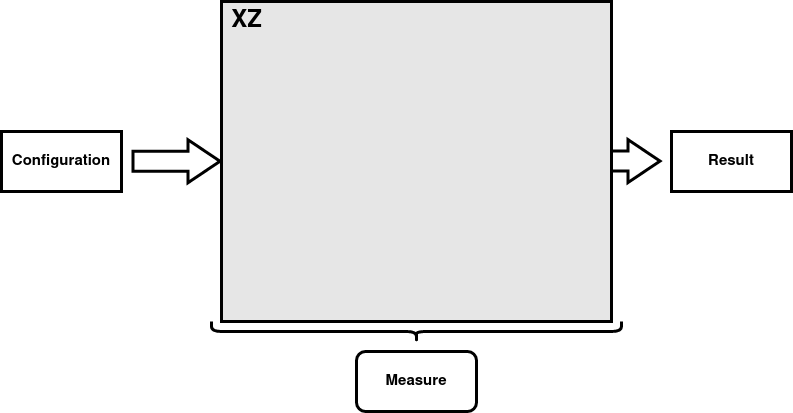
\includegraphics[scale=0.6]{gfx/BlackBoxXZ.png}
    \caption{A Black-box Version of XZ}
    \label{fig:BBxz}
\end{figure}

As an example for a black-box analysis we modify XZ from \autoref{fig:xz}. To perform a black-box analysis, we use XZ with the different configuration that
contain the features to be measured. Now, for each configuration, we observe the non-functional properties we are interested in, such as time spent during the 
execution of the system. During this time, we are unaware on how XZ produces these results, since we can solely observe the effects of XZ  
on the machine on which it is running.
After repeating this process several times, we use all the collected measurements to build a performance-influcence model representing XZ. 

\subsection{Disadvantages of black-box model}
Although a black-box analysis is inherently simple, it faces two major challenges, combinatorial explosion and multicollinear features, both of which
must be handled carefully to build an accurate performance-influence model.

\paragraph{Combinatorial Explosion}
One of the larger problems we face when using black-box analysis is the issue of combinatorial explosion, 
which refers to the effect that when features increase linearly, the number of possible configuration, and hence system variants,
increase exponentially \cite{Combinatorial-explosion}.

Suppose we have a configurable system where each feature is a binary option that you can either select or deselect. We also define 
that in this system each feature is completely independent of another (i.e. the system has no constraints and selecting or deselecting one feature
has no effect on other features). The number of unique configurations this system can produce is $2^n$, where $2$ refers to
the type of feature options allowed, binary in our case, and $n$ denotes the number of features. 

Here is the problem, because all these different features can interact with each other in different ways, and for very small systems
we can certainly brute-force our way by benchmarking all possible configuration, however this does not scale, and certainly not feasible for 
larger systems. For example, the Linux kernel contains 10,000 different features \cite{Linux-Kernel}, for reference it is estimated that the universe
contains about $10^{79}$ atoms, which is still less than the number of variants a system with 263 features produces, it is already impossible to use brute-force to analyze
such a system, let alone the Linux kernel.

For this reason, we cannot fully explore the entire configuration space 
and therefore must select a subset that represent the system with a high accuracy. To achieve this state of the art black-box analyzes use sampling
strategies to find a suitable subset, such as pair-wise sampling, most-enabled-disabled and random sampling.

\paragraph{Multicollinear Features}\label{ColinearF}
We have already mentioned that features that do not influence each other are called independent features, but configurable systems are not composed
of independent features only. If there is a dependence between more than two features, we call these features multicollinear.

The reason why multicollinearity is a problem in a black-box analysis is
that we can only observe nun-functional properties during execution and are not able to correctly assign the influence of each feature
on the system. One way multicollinearity is introduced into a system is by using alternative groups, since the selection of a feature in the
alternative group depends on which features are deselected. \cite{Multicollinearity}

\begin{table}[h]
    \centering
    \begin{tabular}{llllll}
    \hline
    Base & A & B & C &  & $\bm{\Pi(*)}$ \\ \hline
    1 & 1 & 0 & 0 &  & $\mathbf{5}$  \\
    1 & 0 & 1 & 0 &  & $\mathbf{10}$  \\  
    1 & 0 & 0 & 1 &  & $\mathbf{15}$  \\\hline
    \end{tabular}  
    \caption{Configuration example illustrating multicollinearity in an alternative group}\label{tab:alternative}
\end{table}

Now consider the example of \autoref{tab:alternative}, where we see a configuration example that contains multicollinear features due to an alternative group.
The example contains a Base feature and 3 features for an alternative A, B, and C, i.e. for each configuration only one of these 3 characteristics can be selected.
This now clearly shows the dependence between these features, because in order for feature C to be selected, B and C needs to be deselected, therefore
$C = 1 - B - C$ needs to be satisfied. 

\begin{align*}
    \Pi(c) &= 0 + 5 \cdot c(A) + 10\cdot c(B) + 20\cdot c(C) \\
    \Pi(c) &= 5 + 10 \cdot c(A) + 5\cdot c(B) + 20\cdot c(C) \\
    \Pi(c) &= 8 + 20 \cdot c(A) + 10\cdot c(B) + 7\cdot c(C) \\
\end{align*}

This leads to multiple performance-influcence model that are accurate with respect to the individual measurement, 
but make completely different statements when compared.
The problem here is that since one child of the alternative must be selected, the others must be deselected. Therefore, we cannot correctly infer the influence
all features has on to the system, as we can see in our example base is attributed $0$, $5$ and $8$. 
These values of base or the selected feature can be set in any ratio as long as the sum of the two values is equal to the measured time.

Another way  multicollinearity is introduced into the system is to have features that are mandatory or connected by a condition. 
If we have features that are mandatory, we cannot distinguish these features with our black-box analysis because they are always selected
together, and we cannot determine the extent to which each feature influences the system. \cite{Multicollinearity}

\begin{algorithm}[h]
    \caption{Equivalence \label{alg:Colinear}}
    \begin{algorithmic}[1]

    \If{$(c \textit{ and }  \lnot d) or (\lnot c \textit{ and } d)$} 
        \State $c,d \gets False$
    \EndIf

    \end{algorithmic}
    \end{algorithm}

By extending the example code from \hyperref[alg:performanceExample]{Algorithm \ref*{alg:performanceExample}} with an additional condition where $C \equiv D$ holds, 
so that either C or D can be selected without the other, we insert the code snippet  \hyperref[alg:Colinear]{Algorithm \ref*{alg:Colinear}} 
after \hyperref[alg:code_insertion]{Algorithm \ref*{alg:code_insertion}}.

Now, if we select a configuration c that contains the features \{\{A\}, \{B\}, \{C\}\} we get multiple {\perfInfluenceModel}s:

\begin{align*}
    \Pi_1(c) &= 1 + 1\cdot c(C) + 1 \cdot c(D) + 1\cdot c(C) \cdot c(D) \\
    \Pi_2(c) &= 1 + 0\cdot c(C) + 0 \cdot c(D) + 3\cdot c(C) \cdot c(D) \\
    \Pi_3(c) &= 1 + 1\cdot c(C) + 2 \cdot c(D) + 0\cdot c(C) \cdot c(D) \\
\end{align*}

In $\Pi_1(c)$ and $\Pi_2(c)$, all features are assigned different values from what we would expect when looking at Algorithm \ref{alg:performanceExample},
while the \perfInfluenceModel of $\Pi_C(c)$ assigns the expected values.

\subsection{Selecting the configuration space}
Software products are constantly being improved, and to add more functionality, the number of optional features is also increased, which also dramatically increases 
the configuration space, but it has already been shown by Tianyin Xu et. al. \cite{TooManyKnobs} that not all features are equally important and that up to
54,1\% of features are rarely set by users.

We take advantage of this knowledge to solve the combinatorial explosion problem by using our domain knowledge to extract the most important
features we are interested in. This also helps us to mitigate the influence of multicollinear features, as we can ensure that the dependencies 
between the selected features are as low as possible when selecting the features to include in our configuration space.

\subsection{Collecting data}
Having decided which features are of interest to us, we can now turn to the question of to collect our data,
which we can then use to create an \perfInfluenceModel.

Since we are using a black-box analysis, our methods are quite limited. AS shown in \autoref{fig:BBxz}, we are not able to investigate what the system does 
in detail and are limited to the properties that we can observe from the outside. 
In this case, we can measure non-functional properties such as time to completion, energy consumption, memory usage, 
computational resources used, and basically any value we can observe when looking at the machine the system is running on. 
If possible, measurements should be repeated at least 30 times to reduce measurement noise during execution \cite{SampleSize}.


\subsection{Creating a Performance-Influence Model using Multiple Linear Regression}
After collecting all of our measurements, we use them to build our \perfInfluenceModel of the system. 

Various approaches are available to build the model, 
 a popular one being is the use of neural networks, but these have significant disadvantages in that the model itself 
loses its explainability and is usually not comprehensible. 

For to these reasons, we decided to use multiple linear regression. Compared to a neural network, the linear model we 
derived is easy for us humans to understand and interpret, since its structure is very similar to that of an \perfInfluenceModel,
and therefore does not require further adaptation.

We use the following formula for linear regression for matrices\cite{Linear-Regression-Performance}:

\begin{align}\label{formula:linReg}
    Y &= \beta_0 + \beta_1 x_1 + \beta_2 x_2 ... \beta_n x_n + \epsilon   \\
    Y &= X \beta + \epsilon \nonumber\\ \nonumber \\ \nonumber
    Y &= \textit{Dependent variable}\\ \nonumber
    X &= \textit{Independent variable}\\ \nonumber
    \beta &= \textit{Regression coefficient}\\ \nonumber
    \epsilon &= \textit{Error} \nonumber
\end{align}

The model is used to estimate the relationships between the independent variables and the dependent variable.
In our case, $Y$ is a vector with n elements, containing the output of our black-box model, 
i.e. the measurements for each configuration in our set of configurations $\mathcal{C}$. 

Our independent variable $X$ is an $n \times m$ matrix, where $n$ is the number of configurations used and $m$ is the number of configurations
in our set of configurations $\mid \mathcal{C} \mid$.
To accommodate feature interactions in this linear model, we add a term for each interaction we want to include. For example,
if we consider the interaction between features $x_i$ and $x_j$ we add the term $\beta_k x_i x_j$. 

What we are interested in are the values of the coefficients $\beta$, since they quantify the influence of each feature or feature interaction
on the whole system. In addition, $\beta_0$ denotes the intercept, which for us represents the influence of the base code, meaning
the part of the code that is executed regardless of the chosen configuration.

The value of each feature in the matrix is either $1$ if the feature is selected, or $0$ if it is not selected. 
If we have numerical features with $l$ different options,
we split this features into $l$ binary features and encode them as an alternative group in our feature model.

All our measurements have a possible error represented by $\epsilon$ \cite{Linear-Regression}. This is the main difference
between the linear regression model and a \perfInfluenceModel.

\subsubsection{Ordinary Least Squares}
Now that we have seen the general formula of multiple linear regression and know what the different components stand for, we still need to figure out 
how to calculate the regression coefficient $\beta$, the values that tell us the influence of each feature. 

For this purpose, we use the ordinary least squares estimator, which is optimal for the class of linear unbiased estimators, 
but is unreliable when the independent variables $X$ contain a high degree of multicollinearity.
The principal of ordinary least squares is to minimize the sum of the squared residuals, where the residual is the difference between
the predicted value of the estimator and the actual value. \cite{Linear-Regression}


\begin{figure}[H]
    \centering
    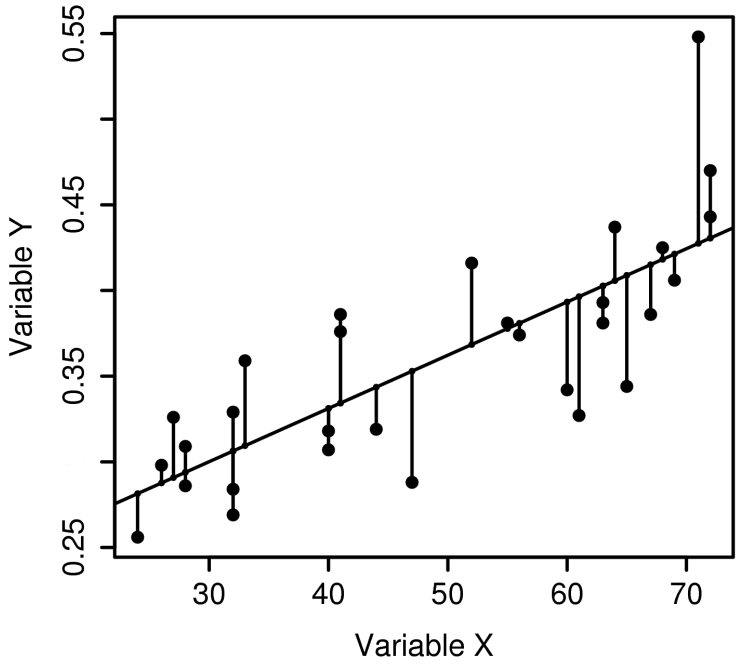
\includegraphics[scale=0.3]{gfx/OLS.png}
    \caption[Ordinary Least Squares regression model residuals]
    {Ordinary Least Squares regression model residuals
    \footnotemark}
    \label{fig:OLS}
\end{figure}
\footnotetext{Visited at 06.03.2023, \url{https://datajobs.com/data-science-repo/OLS-Regression-[GD-Hutcheson].pdf}}

An illustration of an ordinary least squares estimator for a linear regression model can be seen in \autoref{fig:OLS}, where we have only one variable 
X and the corresponding measurements Y, allowing us to compute the single regressor for this linear regression model.

To compute the regression coefficients using ordinary least squares, the following formula is used \cite{Linear-Regression}:

\begin{align}
    \hat{\beta} &=  (\textit{X}^{\top } \textit{X} )^{-1}\textit{X}^{\top} Y \\ \nonumber \\\nonumber
    \hat{\beta} &= \textit{Ordinary Least Squares estimator}\\\nonumber
    \top &= \textit{Matrix Transposed}\nonumber
\end{align}\label{equ:ols}

Now $\hat{\beta}$ contains the regression coefficient we are interested in.

As an example, we can refer to our code from \hyperref[alg:performanceExample]{Algorithm \ref*{alg:performanceExample}}
and sample some configurations to build a multiple linear regression model using ordinary least squares.

\begin{table}[H]
    \centering
    \begin{tabular}{llllllll}
    \hline
    Base & A & B & C & A $\land$ B & A $\land$ C &  & $\bm{\Pi(*)}$ \\ \hline
    1    & 0 & 0 & 0 & 0           & 0           &  &  $\mathbf{1}$   \\
    1    & 1 & 0 & 0 & 0           & 0           &  &  $\mathbf{2}$   \\
    1    & 0 & 1 & 0 & 0           & 0           &  &   $\mathbf{3}$  \\  
    1    & 0 & 0 & 1 & 0           & 0           &  &   $\mathbf{2}$  \\  
    1    & 1 & 1 & 0 & 1           & 0           &  &   $\mathbf{6}$   \\
    1    & 1 & 0 & 1 & 0           & 1           &  &   $\mathbf{3}$  \\  
    1    & 0 & 1 & 1 & 0           & 0           &  &   $\mathbf{4}$  \\  
    1    & 1 & 1 & 1 & 1           & 1           &  &   $\mathbf{7}$  \\ \hline

    \end{tabular}  
    \caption{Configuration samples of \hyperref[alg:performanceExample]{Algorithm \ref*{alg:performanceExample}}}\label{tab:alternative}
\end{table}

Using the configuration samples from \autoref{tab:alternative} we can now determine $\textit{X}$ and $\textit{Y}$:

\begin{displaymath}
    \textit{X} = 
    \begin{bmatrix} 
        1 & 0 & 0 & 0 & 0 & 0 \\
        1 & 1 & 0 & 0 & 0 & 0 \\
        1 & 0 & 1 & 0 & 0 & 0 \\
        1 & 0 & 0 & 1 & 0 & 0 \\
        1 & 1 & 1 & 0 & 1 & 0 \\
        1 & 1 & 0 & 1 & 0 & 1 \\
        1 & 0 & 1 & 1 & 0 & 0 \\
        1 & 1 & 1 & 1 & 1 & 1 
      \end{bmatrix}
      ,
      \textit{Y} =
      \begin{bmatrix}
        1 \\
        2 \\
        3 \\
        2 \\
        6 \\
        3 \\
        4 \\
        7 
      \end{bmatrix}
\end{displaymath}


Using the ordinary least squares \hyperref[equ:ols]{Equation \ref*{equ:ols}}  we obtain the following results:

\begin{equation}
    \hat{\beta} = 1 + 
    \begin{bmatrix}
        0 \\
        1 \\
        2 \\
        1 \\
        2 \\
        0
    \end{bmatrix}
\end{equation}

All values have been rounded to 2 decimal places. 
We can see that all values have been assigned correctly, except for the base feature, which has been assigned 0. The reason for this is that in every
configuration we use, the base feature is active, which is why ordinary least squares assigns the value of the base to the intercept and not $\beta_1$. 

Now we can use the values to create the \perfInfluenceModel:

\begin{equation}
    \Pi = 1 + 1 \cdot A + 2 \cdot B + 1 \cdot C + 2 \cdot A \cdot B + 0 \cdot A \cdot C
\end{equation}

We are aware that if our configurations contains multicollinearity then the ordinary least squares estimator is unreliable.
To check for multicollinearity we use the variance inflation factor (VIF), where a VIF factor of 0 indicates
that there is no multicollinearity in our configurations and the thresholds of 5 and 10 indicate moderate and highly problematic multicollinearity 
respectively. \cite{Multicollinearity}

We compute the VIF using the following equation:

\begin{align}
    VIF_{j} &= \frac{1}{1 - R^{2}_{j}}  \\ \nonumber\\
    R^{2}_{j} &= 1 - \frac{\sum\limits_{\forall c \in \mathcal{T}} (c(o_j) - \overline{c}(o_j))} {\sum\limits_{\forall c \in \mathcal{T}}c(o_j) - {c}(o_j)}
\end{align}

Where $\mathcal{T}$ is the trainings set containing j features $o_j$. The VIF$_{j}$ can be calculated for each feature by using the coefficient
of determination $R^2$. To do this, we need to calculate $R^2$ for each feature $o_j$, fitting a linear regression function $f_j$ to predict whether $o_j$
is selected in the configuration $c \setminus o_j$, using all other features as predictors. /cite{Multicollinearity}
